\documentclass[11pt]{article}

\usepackage[letterpaper, bottom=2cm, right=2cm]{geometry}
\geometry{margin=2cm}

\usepackage{amssymb,amsmath,amsthm} % Símbolos matemáticos
\usepackage[english]{babel}
\usepackage[utf8]{inputenc} % Acentos y otros símbolos 
\usepackage{enumerate}

\usepackage{graphicx}
\DeclareGraphicsExtensions{.pdf}
\pdfcompresslevel=9  % Maximum compression
\pdfobjcompresslevel=3

\usepackage{placeins}
\usepackage{booktabs}
\usepackage{etoolbox}
\usepackage{bbm}
\usepackage{tocloft}
\usepackage{etoc}
\usepackage{setspace}
\usepackage{caption}
\usepackage{subcaption}
\usepackage{ifdraft}
\usepackage{comment}
\usepackage{lscape}
\usepackage{pdfcomment}

\usepackage[looser]{newpxtext} % LOOSER = BETTER WORD SPACE

%\AtBeginEnvironment{table}{\scriptsize}
\AtEndEnvironment{table}{\vspace{0.2in}}

\AtEndEnvironment{figure}{\vspace{0.2in}}

% Para eliminar guiones y justificar texto
\tolerance=1
\emergencystretch=\maxdimen
\hyphenpenalty=10000
\hbadness=10000

\linespread{1.5} 

\let\oldfootnote\footnote % Deja espacio entre el número del pie de página y el inicio del texto
\renewcommand\footnote[1]{%
\oldfootnote{\hspace{0.05mm}#1}}

\renewcommand{\thefootnote} {\textcolor{black}{\arabic{footnote}}} % Súperindice a color negro

\setlength{\footnotesep}{0.75\baselineskip} % Espaciado entre notas al pie

\usepackage{fnpos} % Footnotes al final de pág.

\usepackage[justification=centering, font=bf, labelsep=period, skip=5pt]{caption} % Centrar captions de tablas y ponerlas en negritas
\usepackage{subcaption}

\usepackage{tabularx} % Big tables
\usepackage{multirow}
\usepackage{adjustbox}
\usepackage{longtable}
\usepackage{lscape}

\usepackage{float} % Float tables

\usepackage{color, soul}
\usepackage[dvipsnames]{xcolor} % Color
% Define Maroon color
\definecolor{Maroon}{RGB}{128,0,0}

\usepackage{natbib}
\bibliographystyle{aer}
\setcitestyle{authoryear,aysep={},yysep={,}}
%\setcitestyle{authoryear,open={(},close={)}} %Citation-related commands
\renewcommand{\bibsection}{\section*{References}}

\usepackage{pgfplots} % Gráficas
\pgfplotsset{compat=newest}
\pgfplotsset{width=7.5cm}
\pgfkeys{/pgf/number format/1000 sep={}}

\usepackage{tgpagella}
\usepackage[T1]{fontenc}

\addto\captionsspanish{
    \renewcommand*{\contentsname}{Contents}
    }

\newcommand{\expectation}{\mathbb{E}}
\newcommand{\indicator}{\mathbbm{1}}
\newcommand{\bluetext}[1]{\textcolor{blue}{#1}}

%Added by Roberto for to do notes
\usepackage{marginnote}
\renewcommand*{\marginfont}{\color{red}\sffamily}
\usepackage[colorinlistoftodos]{todonotes}
%\setuptodonotes{fancyline, color=yellow}

\newcommand{\smalltodo}[2][]
{\todo[caption={#2}, #1]
{\begin{spacing}{0.5}#2\end{spacing}}}
%\setlength{\marginparwidth}{2cm}

% https://mirror.hmc.edu/ctan/macros/latex/contrib/todonotes/todonotes.pdf
\newcounter{todoListItems}
\newcommand{\todoLink}[2][ ]{
% Increment counter
\addtocounter{todoListItems}{1}
\todo[%
caption={\protect\hypertarget{todo\thetodoListItems}{}Translation},
#1]
{
#2 \hfill
\hyperlink{todo\thetodoListItems}{$\uparrow$}
}
}

\newcommand{\td}{\todoLink}
\newcommand{\forMW}[1]{\td[color=green!20,inline,caption={\thetodoListItems:
    For @Maria}]{\textbf{@Maria} -- #1}}
\newcommand{\forRG}[1]{\td[color=blue!20,inline,caption={\thetodoListItems:
    For @Roberto}]{\textbf{@Roberto} -- #1}}
\newcommand{\forES}[1]{\td[color=red!20,inline,caption={\thetodoListItems:
    For @Enrique}]{\textbf{@Enrique} -- #1}}
\newcommand{\forAll}[1]{\td[color=orange!20,inline,caption={\thetodoListItems:
    For All}]{\textbf{@All} -- #1}}

\newcommand{\notes}[1]{\footnotesize{#1}}

\definecolor{ultramarine}{RGB}{4,55,242}

\definecolor{LinkBlue}{RGB}{0,35,200}

% For capitalizing first letter referencing sections
\addto\extrasenglish{
    \def\sectionautorefname{Section}
}
 
\usepackage{hyperref} % Hipervínculos en el índice

% Set up configurations for hyperreferences
\hypersetup{colorlinks=true, breaklinks=true, citecolor=Maroon, linkcolor=LinkBlue, menucolor=Maroon, urlcolor=Maroon}

% Find the tables/figures produced by the Stata pipeline (same search order as
% the main paper): local paper/{figures,tables}/ first.
\graphicspath{{./figures/}{../../Protest_Work/results/figures/}}
\makeatletter
\providecommand*{\input@path}{}
\edef\input@path{{./tables/}{../../Protest_Work/results/tables/}\input@path}
\makeatother
\pdfminorversion=7
\DeclareGraphicsExtensions{.pdf,.png}

\title{Violent Effects of Apex Corruption:\\[2pt] Robustness to Including Venezuela}
\author{}
\date{}

\begin{document}
\maketitle

The main analysis (\texttt{violent-effects-of-apex-corruption-main.tex}) excludes Venezuela's scandals throughout. This note re-estimates the paper's core evidence \emph{keeping} Venezuela, changing nothing else: the outcomes (daily violent and peaceful protest counts), the fixed effects (country-by-year, month-of-year, day-of-week), the clustering (country $\times$ year $\times$ day-bin), the sample period (2008--2018), and the event-window widths are all as in the paper. For the democracy splits the terciles are recomputed over the set of countries with a 2008 V-Dem score \emph{including} Venezuela. The headline pattern is unchanged: apex corruption scandals raise violent protests while the peaceful margin and the non-apex partition remain flat.

\section{Apex vs.\ Non-Apex interaction (main-text Table~1)}

\autoref{tab:ven_interaction} re-runs the pooled two-group interaction, which tests whether the post-scandal effect differs between apex and non-apex scandals.

\begin{table}[htb!]
    \caption{Apex vs.\ Non-Apex interaction, Venezuela included.}
    \label{tab:ven_interaction}
    \begin{center}\scriptsize{{
\def\sym#1{\ifmmode^{#1}\else\(^{#1}\)\fi}
\begin{tabular}{l*{6}{c}}
\toprule
            &\multicolumn{2}{c}{$\pm 30$-Day Window}    &\multicolumn{2}{c}{$\pm 60$-Day Window}    &\multicolumn{2}{c}{$\pm 90$-Day Window}    \\\cmidrule(lr){2-3}\cmidrule(lr){4-5}\cmidrule(lr){6-7}
            &\multicolumn{1}{c}{(1)}&\multicolumn{1}{c}{(2)}&\multicolumn{1}{c}{(3)}&\multicolumn{1}{c}{(4)}&\multicolumn{1}{c}{(5)}&\multicolumn{1}{c}{(6)}\\
            &\multicolumn{1}{c}{\shortstack{Violent\\Protests}}&\multicolumn{1}{c}{\shortstack{Peaceful\\Protests}}&\multicolumn{1}{c}{\shortstack{Violent\\Protests}}&\multicolumn{1}{c}{\shortstack{Peaceful\\Protests}}&\multicolumn{1}{c}{\shortstack{Violent\\Protests}}&\multicolumn{1}{c}{\shortstack{Peaceful\\Protests}}\\
\midrule
Post $\times$ Apex&       0.043\sym{**} &      -0.008         &       0.033\sym{**} &      -0.007         &       0.017\sym{*}  &      -0.002         \\
            &     (0.018)         &     (0.013)         &     (0.013)         &     (0.008)         &     (0.010)         &     (0.009)         \\
Post $\times$ Non-Apex&      -0.005         &       0.018         &       0.002         &       0.006         &       0.003         &      -0.001         \\
            &     (0.007)         &     (0.012)         &     (0.006)         &     (0.012)         &     (0.006)         &     (0.009)         \\
\midrule
p-value: Apex $=$ Non-Apex&       0.036         &       0.217         &       0.064         &       0.399         &       0.242         &       0.883         \\
p-value: Apex $>$ Non-Apex (one-sided)&       0.018         &       0.892         &       0.032         &       0.801         &       0.121         &       0.559         \\
Mean (Pre-Scandal)&       0.022         &       0.052         &       0.023         &       0.054         &       0.026         &       0.054         \\
Observations&       11590         &       11590         &       22990         &       22990         &       34390         &       34390         \\
Number of Scandals&         190         &         190         &         190         &         190         &         190         &         190         \\
R-squared   &       0.158         &       0.457         &       0.146         &       0.385         &       0.120         &       0.336         \\
\bottomrule
\end{tabular}
}
}\end{center}
    \footnotesize{OLS estimates of $\beta_{\text{Apex}}$ and $\beta_{\text{Non-Apex}}$ (the post-scandal indicator interacted with Apex and Non-Apex flags), on violent and peaceful protest counts at the $\pm$30/60/90-day windows, on the full scandal panel \emph{including Venezuela}. ``$p$-value: Apex $=$ Non-Apex'' is the two-sided test of equality; the one-sided row tests Apex $>$ Non-Apex. Country-by-year, month-of-year and day-of-week fixed effects; standard errors clustered at the country $\times$ year $\times$ day-bin level. Sample period 2008--2018. Significance: $^{*}$ $p<0.1$, $^{**}$ $p<0.05$, $^{***}$ $p<0.01$.}
\end{table}

\section{Protest dynamics (main-text Figure~1)}

\autoref{fig:ven_dynamics} re-estimates the subsample event studies ($\pm 60$-day window, 15-day bins), keeping Venezuela.

\begin{figure}[htb!]
    \caption{Protest dynamics, Venezuela included ($\pm 60$-day window, 15-day bins).}
    \label{fig:ven_dynamics}
    \begin{center}
    \begin{subfigure}{0.48\textwidth}\caption{Violent, Apex.}
        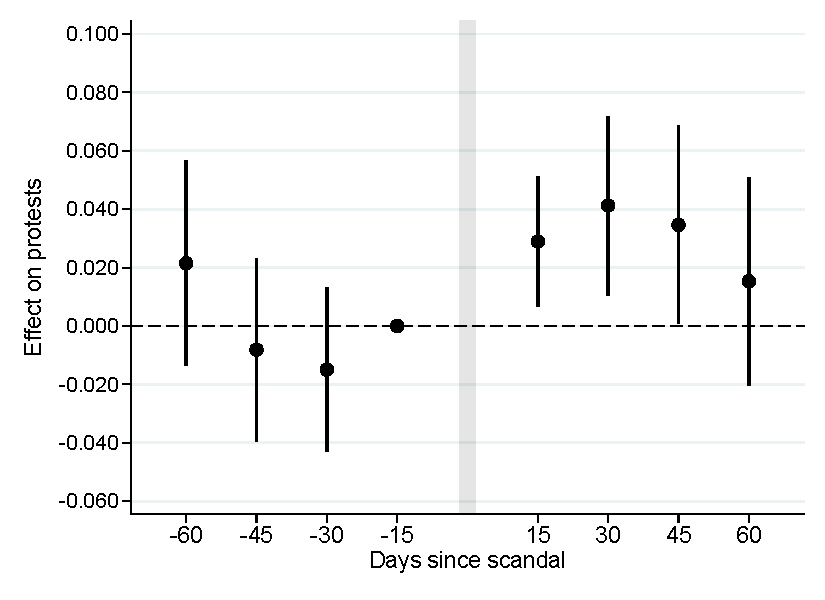
\includegraphics[width=\textwidth]{es_ven_violent_pa.pdf}\end{subfigure}\hfill
    \begin{subfigure}{0.48\textwidth}\caption{Peaceful, Apex.}
        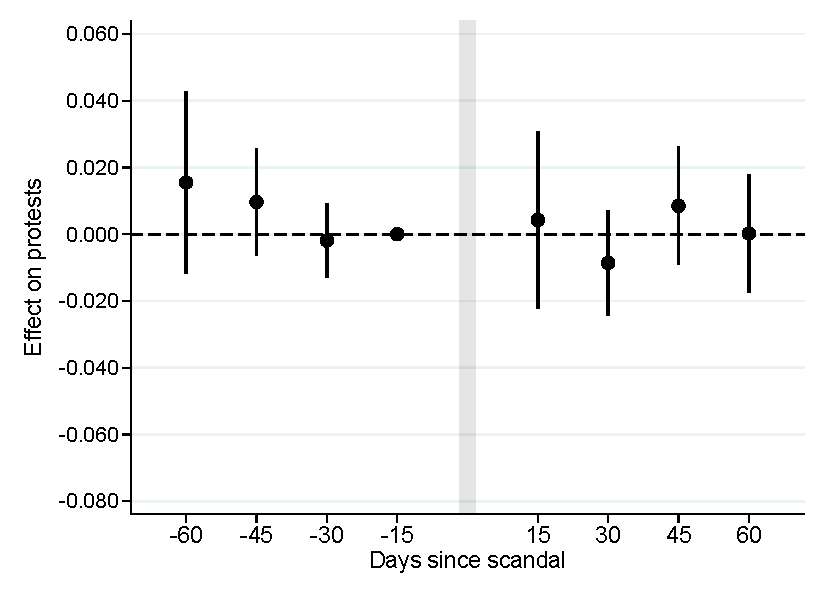
\includegraphics[width=\textwidth]{es_ven_peaceful_pa.pdf}\end{subfigure} \\[4pt]
    \begin{subfigure}{0.48\textwidth}\caption{Violent, Non-Apex.}
        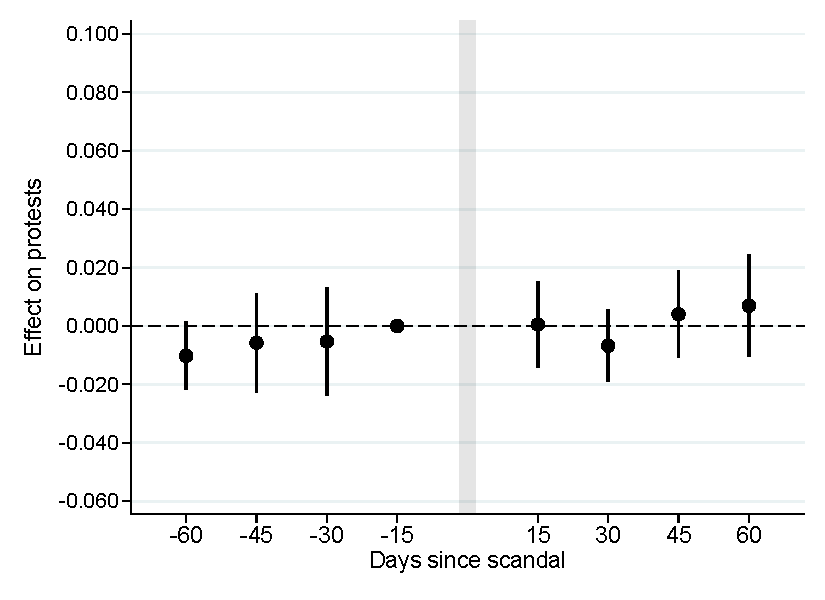
\includegraphics[width=\textwidth]{es_ven_violent_na.pdf}\end{subfigure}\hfill
    \begin{subfigure}{0.48\textwidth}\caption{Peaceful, Non-Apex.}
        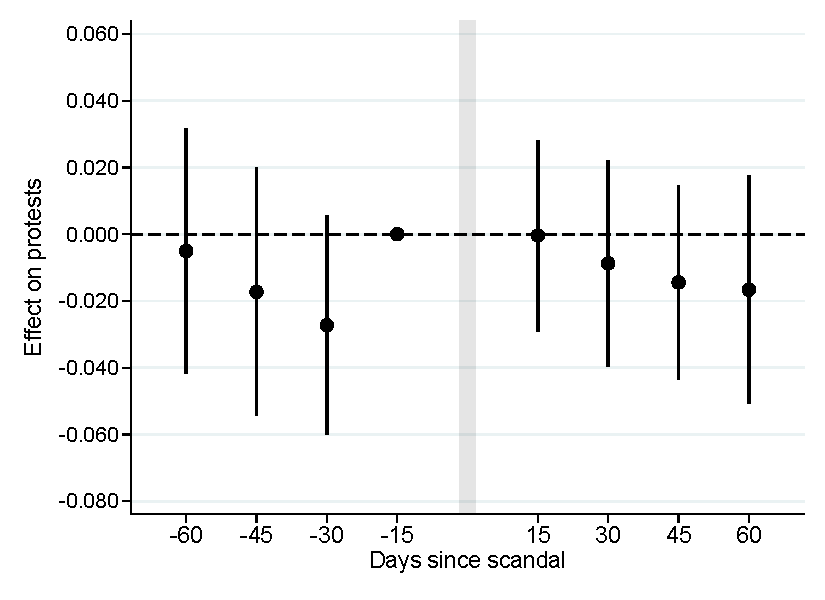
\includegraphics[width=\textwidth]{es_ven_peaceful_na.pdf}\end{subfigure}
    \end{center}
    \footnotesize{Event-time coefficients (points) with 90\% confidence intervals (spikes); the bin immediately before disclosure ($[-15,-1]$ days) is the omitted reference. Estimated on the apex (top) and non-apex (bottom) subsamples, for violent (left) and peaceful (right) protests, \emph{including Venezuela}. Same fixed effects and clustering as \autoref{tab:ven_interaction}. Sample period 2008--2018.}
\end{figure}

\section{Main effect and benchmarks (main-text Table~2)}

\autoref{tab:ven_main} re-estimates the headline effect on the apex and non-apex subsamples, alongside the football-loss and currency-depreciation benchmarks, keeping Venezuela in every panel.

\begin{table}[htb!]
    \caption{Main effect and benchmarks, Venezuela included.}
    \label{tab:ven_main}
    \begin{center}\scriptsize{{
\def\sym#1{\ifmmode^{#1}\else\(^{#1}\)\fi}
\begin{tabular}{l*{6}{c}}
\toprule
&\multicolumn{2}{c}{$\pm 30$-Day Window}    &\multicolumn{2}{c}{$\pm 60$-Day Window}    &\multicolumn{2}{c}{$\pm 90$-Day Window}    \\\cmidrule(lr){2-3}\cmidrule(lr){4-5}\cmidrule(lr){6-7}
&\multicolumn{1}{c}{(1)}&\multicolumn{1}{c}{(2)}&\multicolumn{1}{c}{(3)}&\multicolumn{1}{c}{(4)}&\multicolumn{1}{c}{(5)}&\multicolumn{1}{c}{(6)}\\
&\multicolumn{1}{c}{\shortstack{Violent\\Protests}}&\multicolumn{1}{c}{\shortstack{Peaceful\\Protests}}&\multicolumn{1}{c}{\shortstack{Violent\\Protests}}&\multicolumn{1}{c}{\shortstack{Peaceful\\Protests}}&\multicolumn{1}{c}{\shortstack{Violent\\Protests}}&\multicolumn{1}{c}{\shortstack{Peaceful\\Protests}}\\
\midrule \multicolumn{7}{l}{\textbf{\textit{Panel A: Apex}}} \\
Post Event  &       0.043\sym{***}&       0.002         &       0.032\sym{**} &      -0.004         &       0.012         &       0.006         \\
&     (0.016)         &     (0.009)         &     (0.014)         &     (0.008)         &     (0.013)         &     (0.010)         \\
\midrule
Mean (Pre-Event)&       0.032         &       0.017         &       0.042         &       0.021         &       0.048         &       0.023         \\
Observations&        4209         &        4209         &        8349         &        8349         &       12489         &       12489         \\
Number of Events&          69         &          69         &          69         &          69         &          69         &          69         \\
R-squared   &       0.268         &       0.068         &       0.241         &       0.043         &       0.230         &       0.069         \\
\midrule
\multicolumn{7}{l}{\textbf{\textit{Panel B: Non-Apex}}} \\
Post Event  &      -0.001         &       0.009         &       0.007         &       0.002         &       0.011\sym{*}  &      -0.004         \\
&     (0.004)         &     (0.009)         &     (0.005)         &     (0.012)         &     (0.006)         &     (0.010)         \\
\midrule
Mean (Pre-Event)&       0.016         &       0.071         &       0.012         &       0.072         &       0.013         &       0.073         \\
Observations&        7381         &        7381         &       14641         &       14641         &       21901         &       21901         \\
Number of Events&         121         &         121         &         121         &         121         &         121         &         121         \\
R-squared   &       0.107         &       0.552         &       0.095         &       0.464         &       0.080         &       0.398         \\
\bottomrule
\multicolumn{7}{l}{\textbf{\textit{Panel C: Football match losses}}} \\
Post Event  &       0.011\sym{*}  &       0.002         &       0.016\sym{**} &       0.004         &       0.012         &       0.010         \\
&     (0.006)         &     (0.011)         &     (0.008)         &     (0.012)         &     (0.008)         &     (0.013)         \\
\midrule
Mean (Pre-Event)&       0.015         &       0.041         &       0.019         &       0.035         &       0.016         &       0.035         \\
Observations&       10370         &       10370         &       20570         &       20570         &       30770         &       30770         \\
Number of Events&         170         &         170         &         170         &         170         &         170         &         170         \\
R-squared   &       0.787         &       0.599         &       0.734         &       0.392         &       0.632         &       0.341         \\
\bottomrule
\multicolumn{7}{l}{\textbf{\textit{Panel D: Currency depreciations}}} \\
Post Event  &       0.010         &      -0.001         &       0.004         &      -0.012\sym{*}  &       0.000         &      -0.012\sym{*}  \\
&     (0.011)         &     (0.008)         &     (0.007)         &     (0.007)         &     (0.007)         &     (0.006)         \\
\midrule
Mean (Pre-Event)&       0.025         &       0.027         &       0.024         &       0.029         &       0.026         &       0.030         \\
Observations&       10004         &       10004         &       19844         &       19844         &       29684         &       29684         \\
Number of Events&         164         &         164         &         164         &         164         &         164         &         164         \\
R-squared   &       0.368         &       0.262         &       0.374         &       0.163         &       0.374         &       0.140         \\
\bottomrule
\end{tabular}
}
}\end{center}
    \footnotesize{Effect of a post-event indicator on violent and peaceful protest counts at the $\pm$30/60/90-day windows, on four samples (apex scandals, non-apex scandals, football-match losses, currency depreciations), \emph{including Venezuela}. Construction as in the main paper's Table~2. Sample period 2008--2018. Significance: $^{*}$ $p<0.1$, $^{**}$ $p<0.05$, $^{***}$ $p<0.01$.}
\end{table}

\section{Heterogeneity by democracy (main-text Tables~3 and~S3)}

Tables~\ref{tab:ven_dem_elec} and~\ref{tab:ven_dem_lib} re-estimate the Low vs.\ Medium+High democracy split, with terciles formed---including Venezuela---from the 2008 V-Dem Electoral and Liberal Democracy Indices, respectively.

\begin{table}[htb!]
    \caption{Effect by 2008 level of democracy (Electoral index), Venezuela included.}
    \label{tab:ven_dem_elec}
    \begin{center}\scriptsize{{
\def\sym#1{\ifmmode^{#1}\else\(^{#1}\)\fi}
\begin{tabular}{l*{6}{c}}
\toprule
            &\multicolumn{2}{c}{$\pm 30$-Day Window}    &\multicolumn{2}{c}{$\pm 60$-Day Window}    &\multicolumn{2}{c}{$\pm 90$-Day Window}    \\\cmidrule(lr){2-3}\cmidrule(lr){4-5}\cmidrule(lr){6-7}
            &\multicolumn{1}{c}{(1)}&\multicolumn{1}{c}{(2)}&\multicolumn{1}{c}{(3)}&\multicolumn{1}{c}{(4)}&\multicolumn{1}{c}{(5)}&\multicolumn{1}{c}{(6)}\\
            &\multicolumn{1}{c}{\shortstack{Violent\\Protests}}&\multicolumn{1}{c}{\shortstack{Peaceful\\Protests}}&\multicolumn{1}{c}{\shortstack{Violent\\Protests}}&\multicolumn{1}{c}{\shortstack{Peaceful\\Protests}}&\multicolumn{1}{c}{\shortstack{Violent\\Protests}}&\multicolumn{1}{c}{\shortstack{Peaceful\\Protests}}\\
\midrule
Post $\times$ Medium+High&       0.017\sym{**} &       0.011         &       0.020\sym{**} &      -0.003         &       0.018\sym{**} &      -0.006         \\
            &     (0.007)         &     (0.008)         &     (0.008)         &     (0.008)         &     (0.008)         &     (0.007)         \\
Post $\times$ Low&       0.006         &       0.003         &       0.001         &       0.008         &      -0.009\sym{*}  &       0.007         \\
            &     (0.007)         &     (0.013)         &     (0.006)         &     (0.017)         &     (0.005)         &     (0.014)         \\
\midrule
p-value: Medium+High $=$ Low&       0.253         &       0.527         &       0.072         &       0.562         &       0.006         &       0.405         \\
p-value: Medium+High $>$ Low (one-sided)&       0.127         &       0.263         &       0.036         &       0.719         &       0.003         &       0.797         \\
Mean (Pre-Scandal)&       0.022         &       0.052         &       0.023         &       0.054         &       0.026         &       0.054         \\
Observations&       11590         &       11590         &       22990         &       22990         &       34390         &       34390         \\
R-squared   &       0.150         &       0.456         &       0.143         &       0.385         &       0.121         &       0.336         \\
\bottomrule
\end{tabular}
}
}\end{center}
    \footnotesize{OLS estimates of $\beta_{\text{Medium+High}}$ and $\beta_{\text{Low}}$ (the post-scandal indicator interacted with the top-two-tercile and bottom-tercile flags of the 2008 V-Dem Electoral Democracy Index), on violent and peaceful protest counts at the $\pm$30/60/90-day windows, \emph{including Venezuela}. Same fixed effects and clustering as above. Sample period 2008--2018. Significance: $^{*}$ $p<0.1$, $^{**}$ $p<0.05$, $^{***}$ $p<0.01$.}
\end{table}

\begin{table}[htb!]
    \caption{Effect by 2008 level of democracy (Liberal index), Venezuela included.}
    \label{tab:ven_dem_lib}
    \begin{center}\scriptsize{{
\def\sym#1{\ifmmode^{#1}\else\(^{#1}\)\fi}
\begin{tabular}{l*{6}{c}}
\toprule
            &\multicolumn{2}{c}{$\pm 30$-Day Window}    &\multicolumn{2}{c}{$\pm 60$-Day Window}    &\multicolumn{2}{c}{$\pm 90$-Day Window}    \\\cmidrule(lr){2-3}\cmidrule(lr){4-5}\cmidrule(lr){6-7}
            &\multicolumn{1}{c}{(1)}&\multicolumn{1}{c}{(2)}&\multicolumn{1}{c}{(3)}&\multicolumn{1}{c}{(4)}&\multicolumn{1}{c}{(5)}&\multicolumn{1}{c}{(6)}\\
            &\multicolumn{1}{c}{\shortstack{Violent\\Protests}}&\multicolumn{1}{c}{\shortstack{Peaceful\\Protests}}&\multicolumn{1}{c}{\shortstack{Violent\\Protests}}&\multicolumn{1}{c}{\shortstack{Peaceful\\Protests}}&\multicolumn{1}{c}{\shortstack{Violent\\Protests}}&\multicolumn{1}{c}{\shortstack{Peaceful\\Protests}}\\
\midrule
Post $\times$ Medium+High&       0.018\sym{***}&       0.016\sym{**} &       0.020\sym{***}&       0.013         &       0.016\sym{**} &       0.008         \\
            &     (0.006)         &     (0.008)         &     (0.007)         &     (0.009)         &     (0.006)         &     (0.008)         \\
Post $\times$ Low&      -0.002         &      -0.012         &      -0.007         &      -0.032\sym{*}  &      -0.013         &      -0.026\sym{*}  \\
            &     (0.008)         &     (0.016)         &     (0.007)         &     (0.017)         &     (0.010)         &     (0.015)         \\
\midrule
p-value: Medium+High $=$ Low&       0.028         &       0.097         &       0.009         &       0.023         &       0.015         &       0.047         \\
p-value: Medium+High $>$ Low (one-sided)&       0.014         &       0.049         &       0.004         &       0.012         &       0.008         &       0.023         \\
Mean (Pre-Scandal)&       0.022         &       0.052         &       0.023         &       0.054         &       0.026         &       0.054         \\
Observations&       11590         &       11590         &       22990         &       22990         &       34390         &       34390         \\
R-squared   &       0.151         &       0.457         &       0.144         &       0.387         &       0.121         &       0.336         \\
\bottomrule
\end{tabular}
}
}\end{center}
    \footnotesize{As \autoref{tab:ven_dem_elec}, but terciles are formed from the 2008 V-Dem Liberal Democracy Index. Sample period 2008--2018.}
\end{table}

\end{document}
